\chapter{Comparative Result}
	
	\section{Used Model's Performance}
	As described in $Methodology$ section, we've used LSTM model here. A quick summery of LSTM performance is as follow. \\
	
	\begin{table}[H]
		\centering
		\begin{tabular}{|l|l|}
			\hline
			Accuracy Type       & Accuracy \\ \hline
			Train Accuracy      & 89.72\%  \\ \hline
			Validation Accuracy & 97.78\%  \\ \hline
			Test Accuracy       & 97.90\%  \\ \hline
		\end{tabular}
		\caption{LSTM Accuracy}
	\end{table}
	
	
	The following figure shows the graph of model's loss during 5 epochs.\\
	
	\begin{figure}[H]
		\centering
		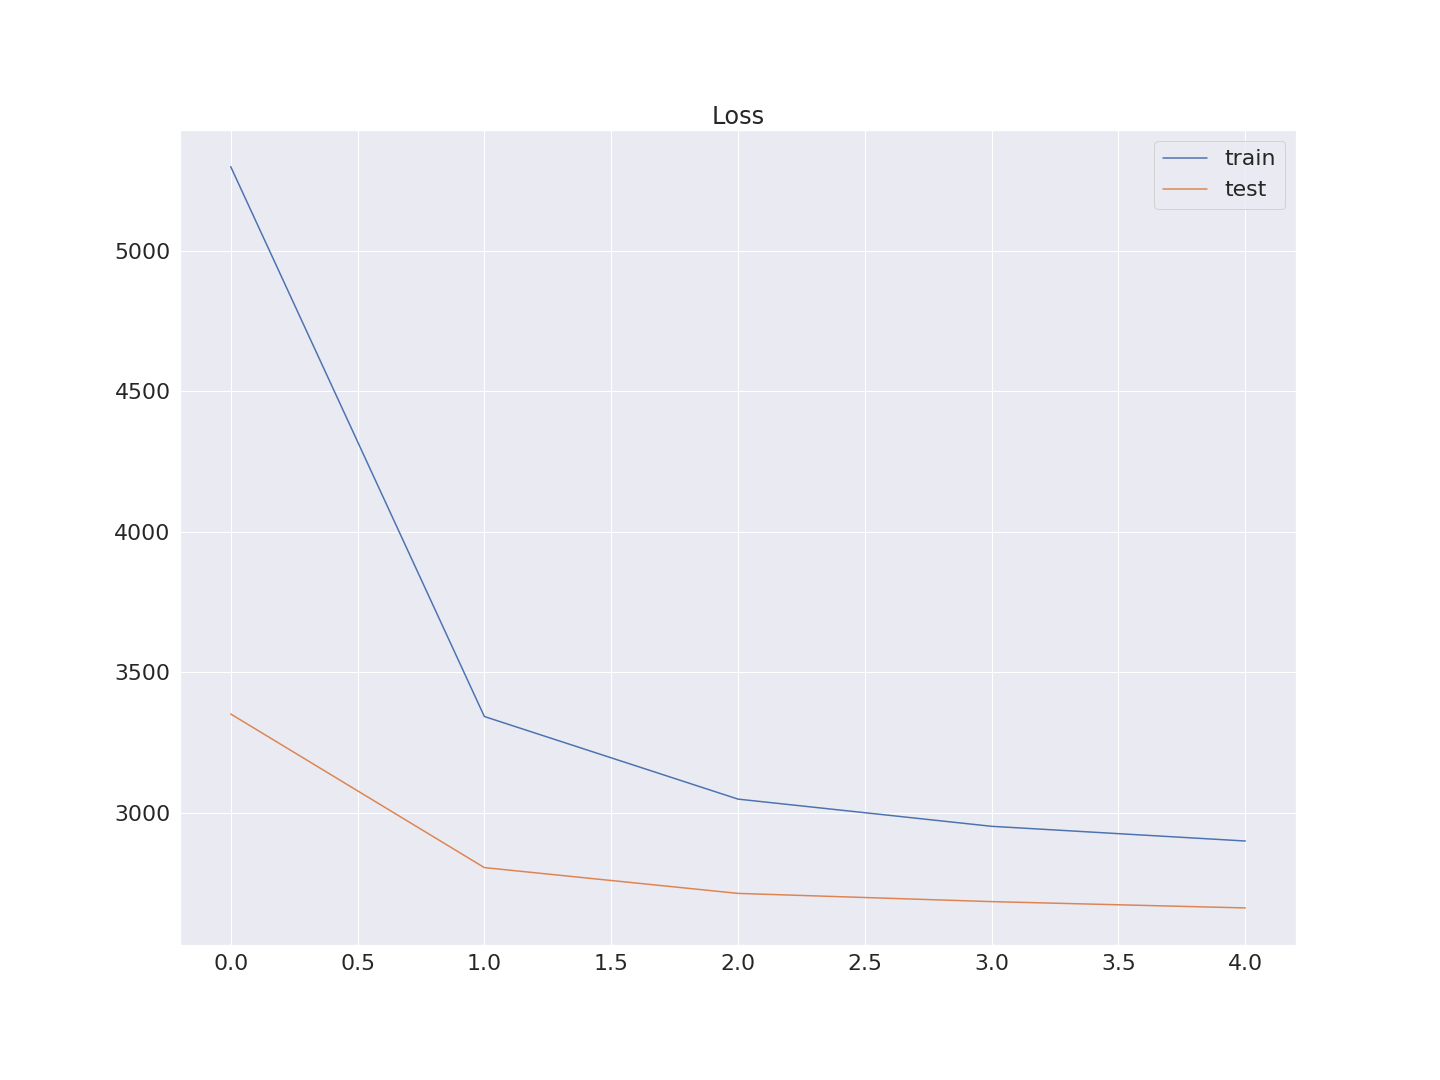
\includegraphics[scale=0.30]{lstm_loss}
		\caption{LSTM Loss Graph}
	\end{figure}
	\vline

	The following figure shows the graph of the model's test accuracy during 5 epochs.\\
	\begin{figure}[H]
		\centering
		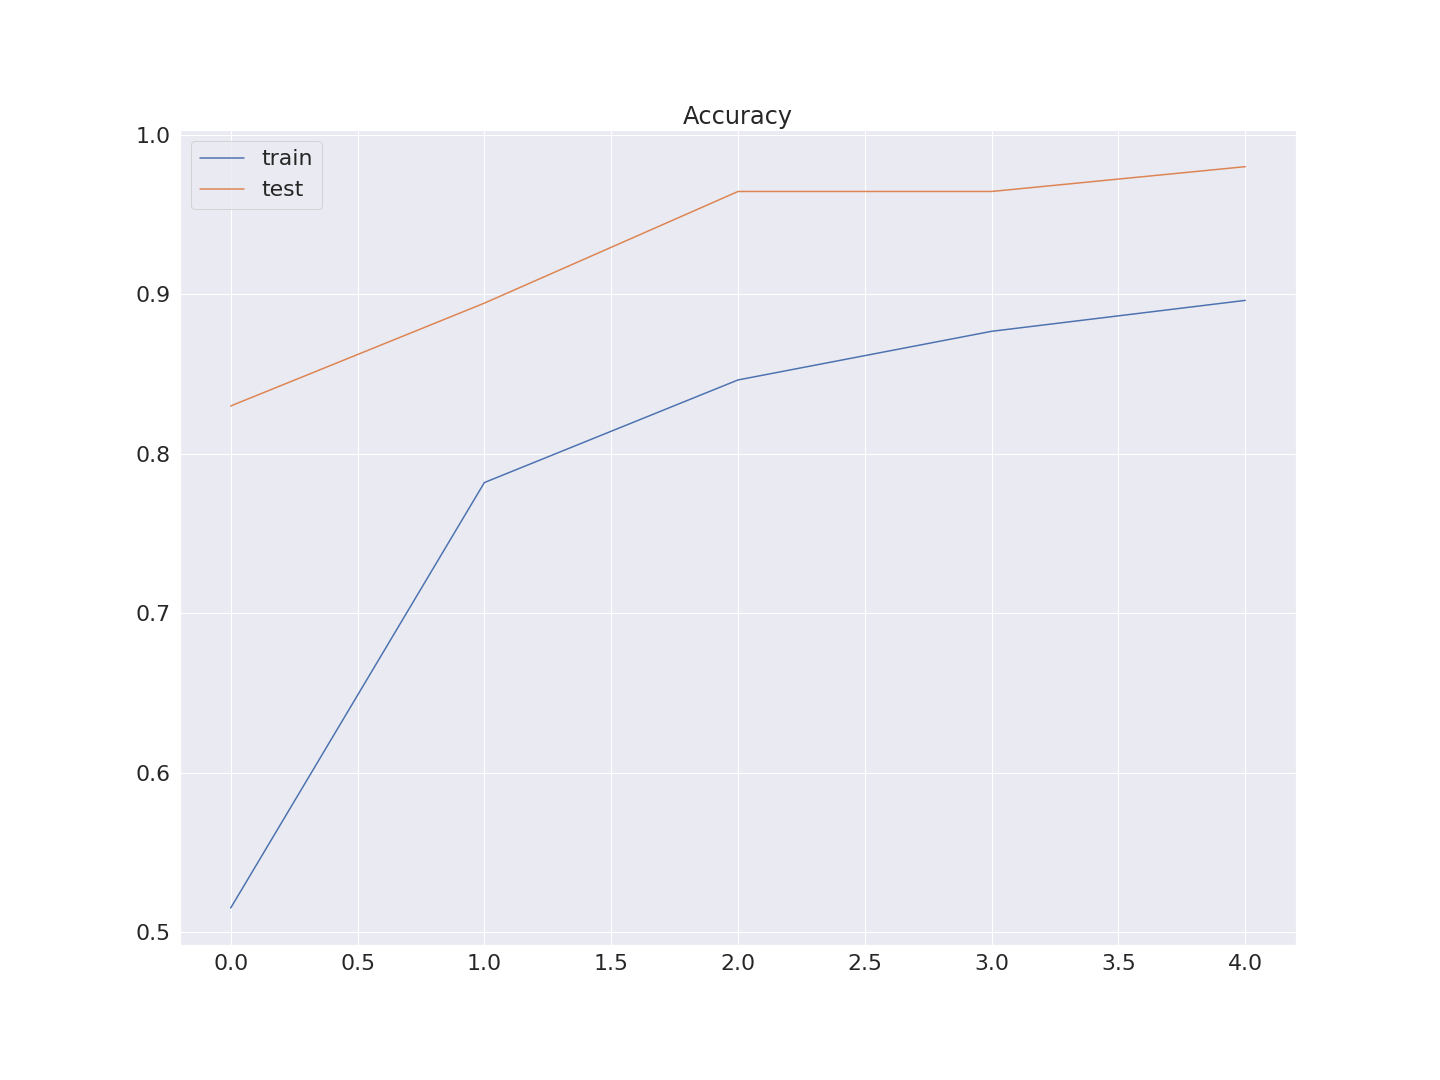
\includegraphics[scale=0.30]{lstm_accuracy}
		\caption{LSTM Accuracy Graph}
	\end{figure}
	\vline
	
	
	\section{Another Model's Performance}
	We try with other two model architecture, RNN and GRU. Here we'll look the performance of these two model. \\
	
		\subsection{RNN Performance}
		A quick summery of RNN model performance is as follow. \\
		
		\begin{table}[H]
			\centering
			\begin{tabular}{|l|l|}
				\hline
				Accuracy Type       & Accuracy \\ \hline
				Train Accuracy      & 57.53\%  \\ \hline
				Validation Accuracy & 63.00\%  \\ \hline
				Test Accuracy       & 63.00\%  \\ \hline
			\end{tabular}
			\caption{RNN Accuracy}
		\end{table}
		
		
		The following figure shows the graph of RNN's loss during 5 epochs.\\
		
		\begin{figure}[H]
			\centering
			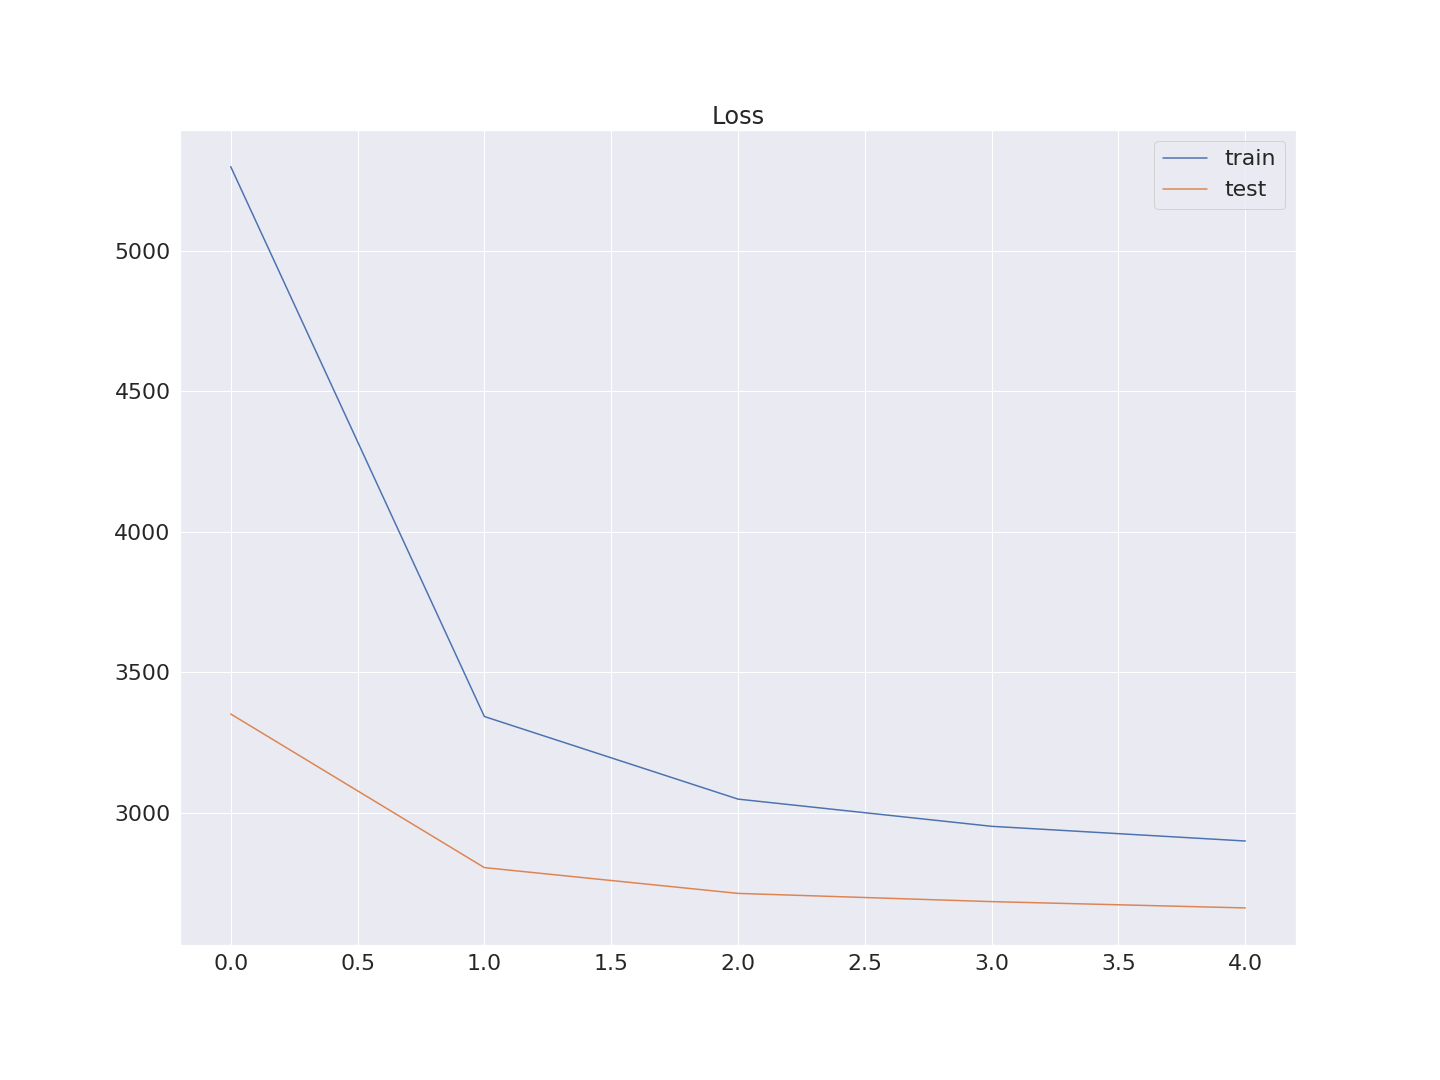
\includegraphics[scale=0.30]{rnn_loss}
			\caption{RNN Loss Graph}
		\end{figure}
		\vline
		
		The following figure shows the graph of RNN's test accuracy during 5 epochs.\\
		\begin{figure}[H]
			\centering
			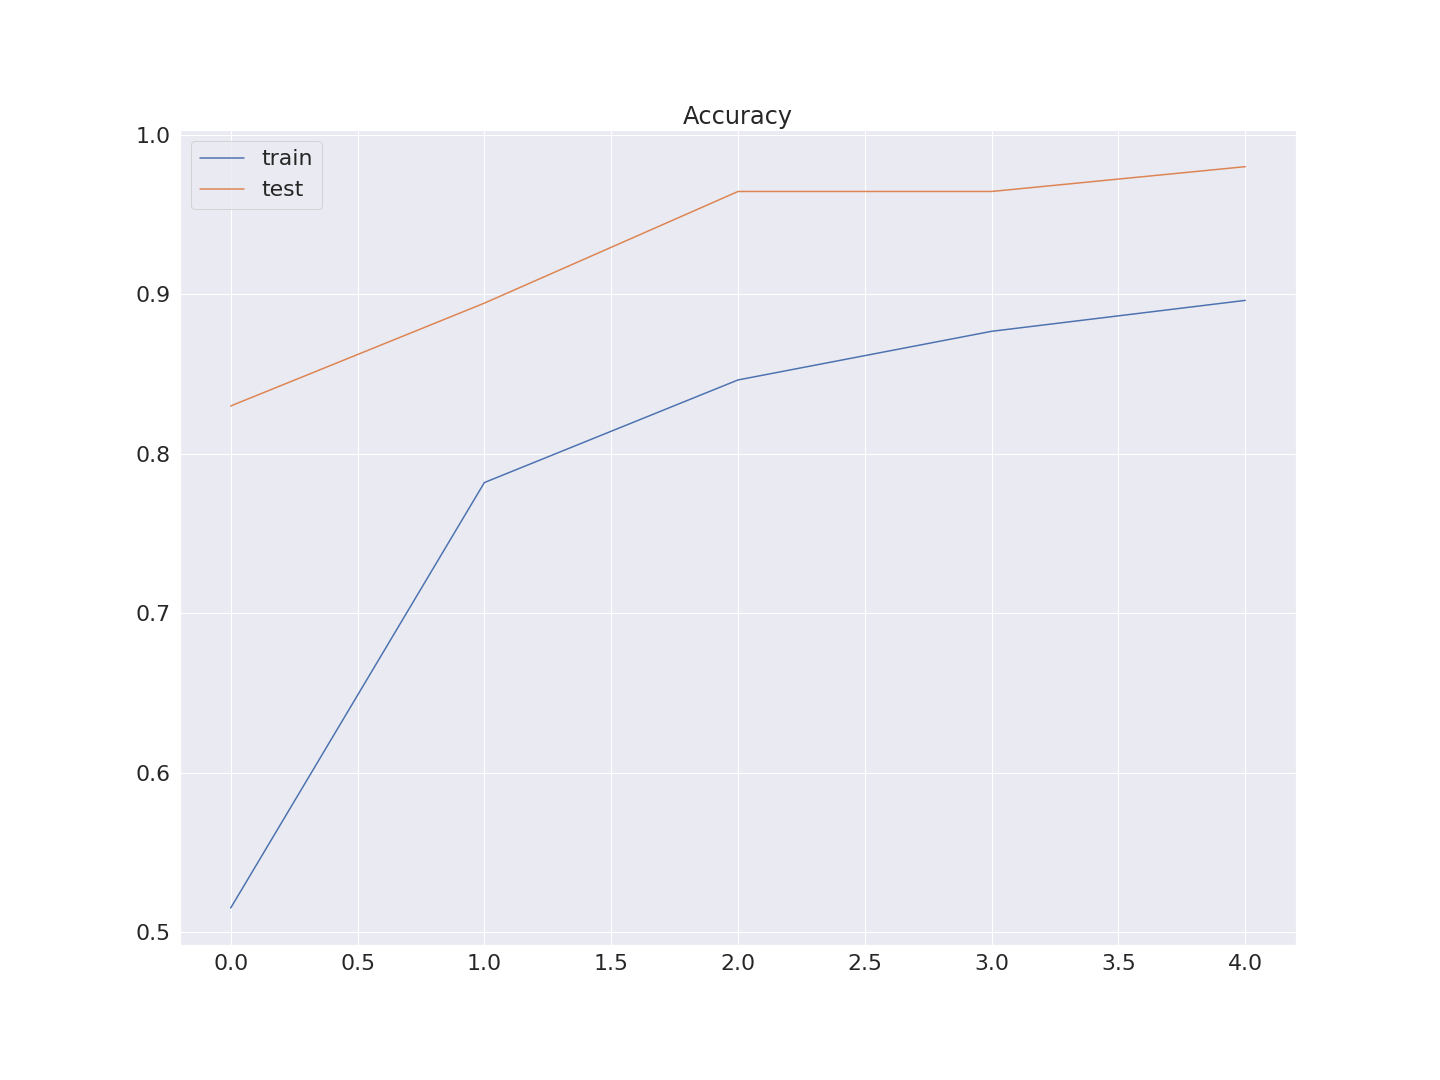
\includegraphics[scale=0.30]{rnn_accuracy}
			\caption{RNN Accuracy Graph}
		\end{figure}
		\vline
		
		
		\subsection{GRU Performance}
		A quick summery of GRU model performance is as follow. \\
		
		\begin{table}[H]
			\centering
			\begin{tabular}{|l|l|}
				\hline
				Accuracy Type       & Accuracy \\ \hline
				Train Accuracy      & 83.59\%  \\ \hline
				Validation Accuracy & 37.30\%  \\ \hline
				Test Accuracy       & 37.30\% \\ \hline
			\end{tabular}
			\caption{GRU Accuracy}
		\end{table}
		
		
		The following figure shows the graph of GRU's loss during 5 epochs.\\
		
		\begin{figure}[H]
			\centering
			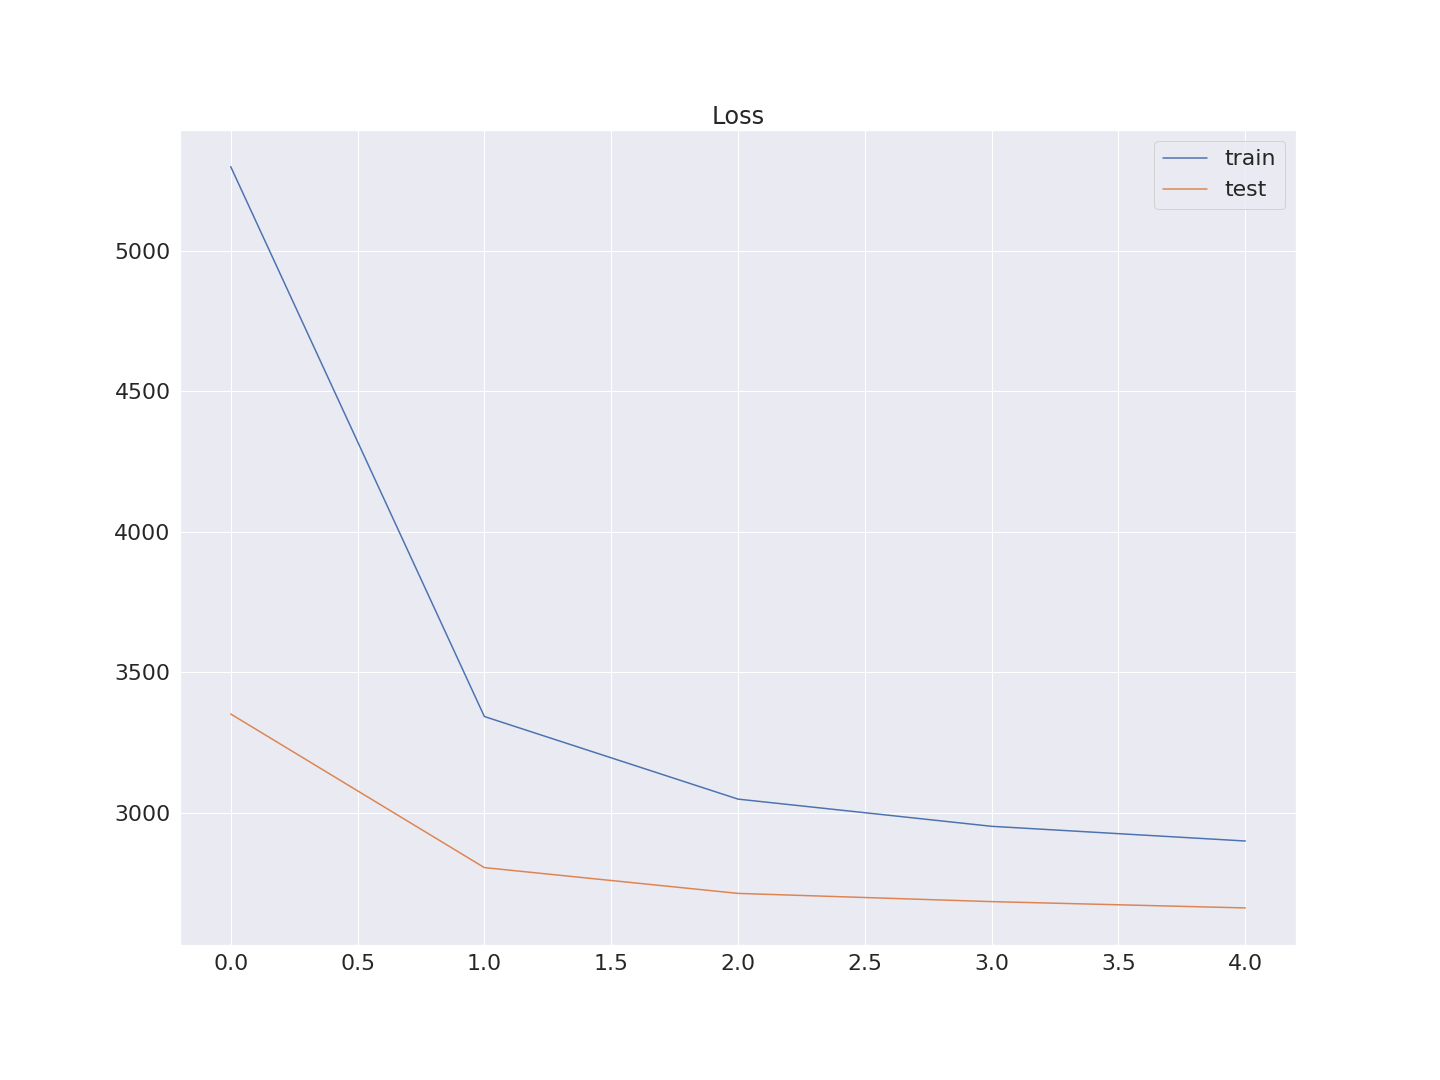
\includegraphics[scale=0.30]{gru_loss}
			\caption{GRU Loss Graph}
		\end{figure}
		\vline
		
		The following figure shows the graph of GRU's test accuracy during 5 epochs.\\
		\begin{figure}[H]
			\centering
			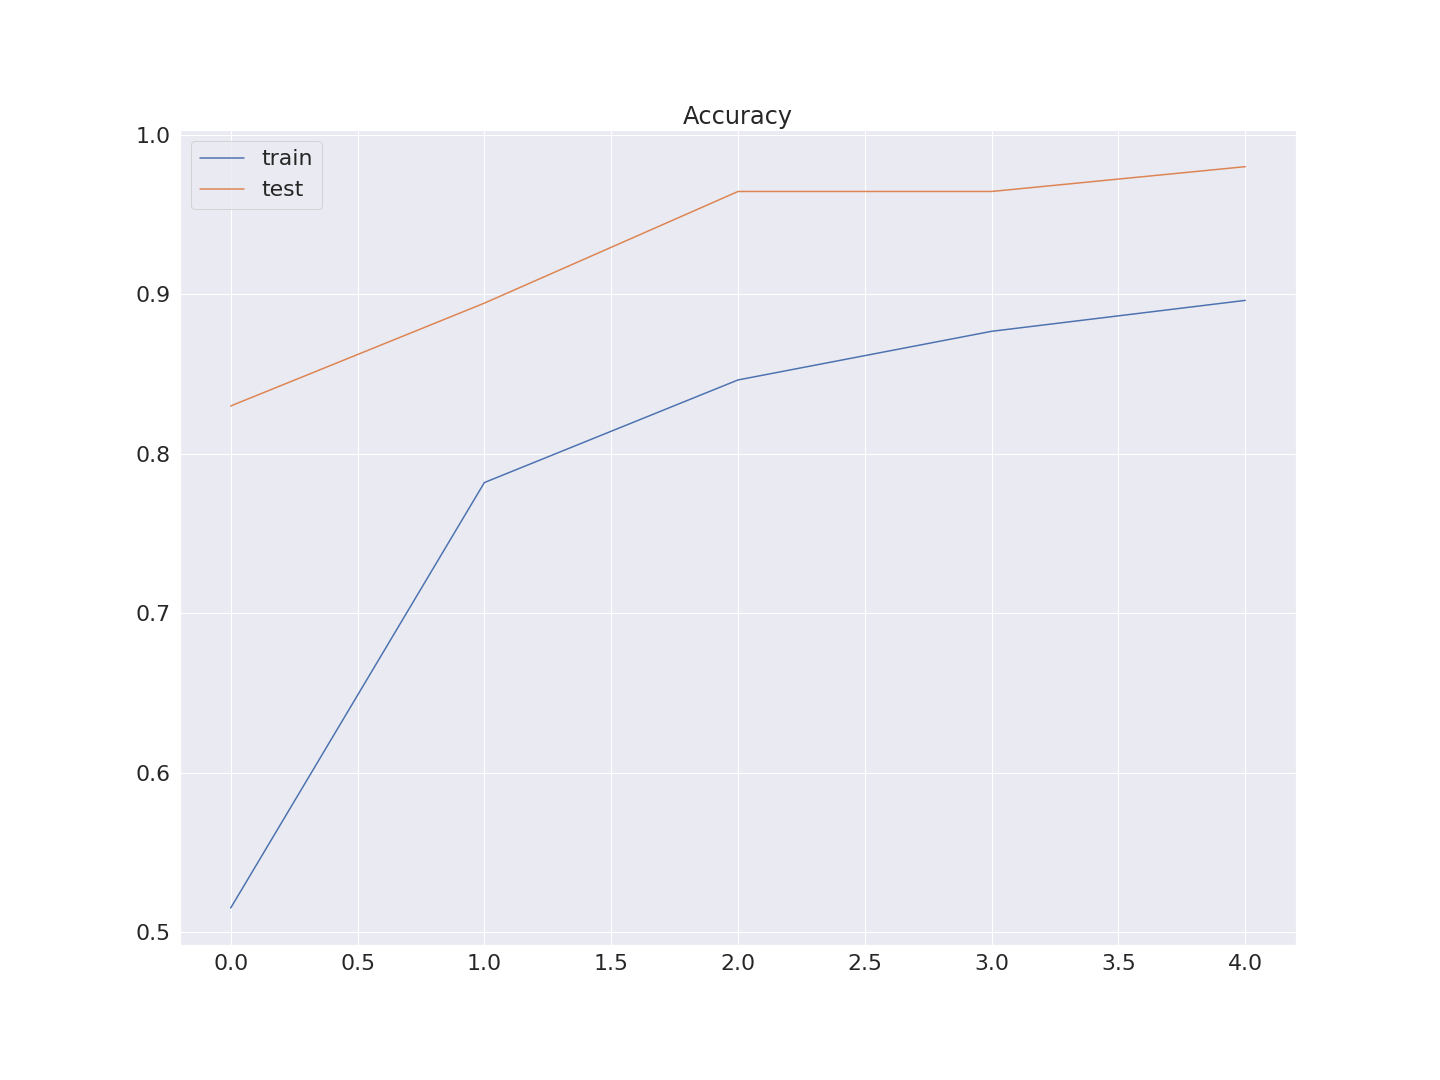
\includegraphics[scale=0.30]{gru_accuracy}
			\caption{GRU Accuracy Graph}
		\end{figure}
		\vline
		
	
	\section{Comparison Altogether}
	Lets have look on both of these model and their accuracy altogether. \\
	
	\begin{table}[H]
		\centering
		\begin{tabular}{|l|l|l|l|}
			\hline
			Accuracy Type \textbackslash Model & LSTM    & RNN     & GRU     \\ \hline
			Train Accuracy                     & 89.72\% & 57.53\% & 83.59\% \\ \hline
			Validation Accuracy                & 97.78\% & 63.00\% & 37.30\% \\ \hline
			Test Accuracy                      & 97.90\% & 63.00\% & 37.30\% \\ \hline
		\end{tabular}
		\caption{Accuracy Comparison Between LSTM, RNN and GRU}
	\end{table}
	
	The table above shows various accuracy comparison between various models. And we can easily see that LSTM is the obvious champion here.